% arara: pdflatex
% !arara: animate: {delay: 80}
% !arara: indent: {overwrite: yes, localSettings: yes}
\documentclass[aspectratio=43,mathserif]{beamer}
%\documentclass[handout,mathserif]{beamer}
\usepackage{caption}
\captionsetup[figure]{font=scriptsize, justification=centering}
\usepackage{amsmath}
\usepackage{booktabs}
\usepackage{etoolbox}
\usepackage{multirow}
\usepackage{pgfplots}
\usepackage[]{media9}
\usepackage[export]{adjustbox}
\usetikzlibrary{positioning}
\usetikzlibrary{fit}
\usetikzlibrary{backgrounds}
\usetikzlibrary{calc}
\usetikzlibrary{shapes}
\usetikzlibrary{mindmap}
\usetikzlibrary{decorations.text}
\pgfplotsset{compat=1.7}
\let\bbordermatrix\bordermatrix
\patchcmd{\bbordermatrix}{8.75}{4.75}{}{}
\patchcmd{\bbordermatrix}{\left(}{\left[}{}{}
\patchcmd{\bbordermatrix}{\right)}{\right]}{}{}

\usepackage[english]{babel}

\usepackage[style=mla,backend=bibtex]{biblatex}

\usetheme[titlepagelogo=figures/fer,
  secondlogo = true,
  thirdlogo = true,
  color=larics,
  language=custom,
  bullet=square,
  ]{TorinoTh}
  
\titlepagesecondlogo{figures/unizg}
\titlepagethirdlogo{figures/larics_light}
\author{Ana Batinović, mag. ing.}
%\setcandidatelabel{Pristupnik/Candidate}
\setcandidatelabel{Candidate}
%\setrellabel{Mentor/Supervisor}
\setrellabel{Supervisor}
\setsubject{PhD Qualifying Exam}
\rel{doc. dr. sc. Tamara Petrović}
\title[PhD Qualifying Exam]{An Overview of Coordinated Exploration Strategies using Multi-Robot Systems}

\ateneo{University of Zagreb \\ Faculty of Electrical Engineering and Computing}
\date{Zagreb, 9 March 2020}
\usepackage{subfigure}
\usepackage{multirow}
\newcommand{\backupbegin}{
   \newcounter{framenumberappendix}
   \setcounter{framenumberappendix}{\value{framenumber}}
}
\newcommand{\backupend}{
   \addtocounter{framenumberappendix}{-\value{framenumber}}
   \addtocounter{framenumber}{\value{framenumberappendix}} 
}

% tikzmark command, for shading over items
\newcommand{\tikzmark}[1]{\tikz[overlay,remember picture] \node (#1) {};}

% standard enumeration
%\setbeamertemplate{enumerate items}{(\arabic{enumi})}

% default itemize
\setbeamertemplate{itemize items}[circle]

% transparency
\setbeamercovered{transparent=15}

% for resuming lists across frames
\newcounter{savedenum}
\newcommand*{\saveenum}{\setcounter{savedenum}{\theenumi}}
\newcommand*{\resume}{\setcounter{enumi}{\thesavedenum}}

% title
\tikzset{
   invisible/.style={opacity=0},
   visible on/.style={alt=#1{}{invisible}},
   alt/.code args={<#1>#2#3}{%
      \alt<#1>{\pgfkeysalso{#2}}{\pgfkeysalso{#3}} % \pgfkeysalso doesn't change the path
   },
}

%\includeonlyframes{daytoday}

% add references
\addbibresource{references.bib}
%naslovna
\begin{document}
\begin{frame}[plain, noframenumbering]
\titlepage
\end{frame}
%sadrzaj prezentacije
\begin{frame}
	\frametitle{Content}
	\begin{itemize}
		\item[1)] Introduction
		\item[2)] Autonomous exploration
		\item[3)] 2D exploration strategies
		\item[4)] 3D exploration strategies
		\item[5)] Conclusion and future work
	\end{itemize}
\end{frame}

%uvod
\begin{frame}
	\frametitle{Introduction}
	\begin{itemize}
		\item[-] \textbf{Autonomous exploration} - the ability of robots to autonomously travel around an unknown environment gathering the necessary information to obtain a useful map for navigation\footcite{Julia2012}
		\item[-] We focuse on different exploration strategies using \textbf{a multi-robot system} with \textbf{coordinated} robots that could accomplish a given task in a way which minimizes the overall exploration time
	\end{itemize}
\end{frame}

\begin{frame}
\frametitle{Multi-robot exploration}
\begin{itemize}
	\item[-] \textbf{ADVANTAGES:}
		\begin{itemize}
			\item[-] Robustness (due to redundancy)
			\item[-] Efficiency (a robot team can accomplish a predefined task much quicker than a single robot can\footcite{Dias2000})
			\item[-] Sensor fusion (can compensate sensor uncertainty\footcite{Wurm2008})
			\item[-] Free from single-point failure (if system is decentralized)
			\item[-] Larger range of task domains\footcite{Dias2006}
		\end{itemize}
	\item[-] \textbf{DISADVANTAGES:}
		\begin{itemize}
		\item[-] High communication requirement in general
		\item[-] If greedy assignment methods are used, convergence to a suboptimal goal is possible
	\end{itemize} 
\end{itemize}
\end{frame}


\begin{frame}
	\frametitle{Autonomous exploration strategies (1)}
			\begin{itemize}
				\item[-] \textbf{Occupancy grid map} - discretizes the environment into a grid of map cells\footcite{Moravec}. Cells can be classified as \textbf{free, occupied or unknown}.
				\item[-] Frontier-based exploration algorithms introduced by Yamauchi\footcite{Yamauchi1997} 				
			\end{itemize}
\end{frame}

\begin{frame}
	\frametitle{Autonomous exploration strategies (2)}
	\begin{figure}
		\centering
		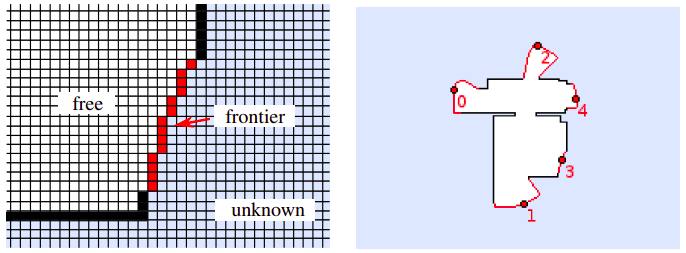
\includegraphics[width=0.8\textwidth]{figures/environment1}
		\caption{2D occupancy grid map: unknown cells are shown light blue, free cells are depicted in white and occupied cells (obstacles) in black. Left: Frontier cells (red) are determined at the boundary between free and unknown map cells. Right: Five exploration targets, visualized as red circles, are generated at frontiers (Source\footcite{Wurm2012})}
	\end{figure}
\end{frame}

\begin{frame}
	\frametitle{Autonomous exploration strategies (3)}
	\begin{figure}
		\centering
		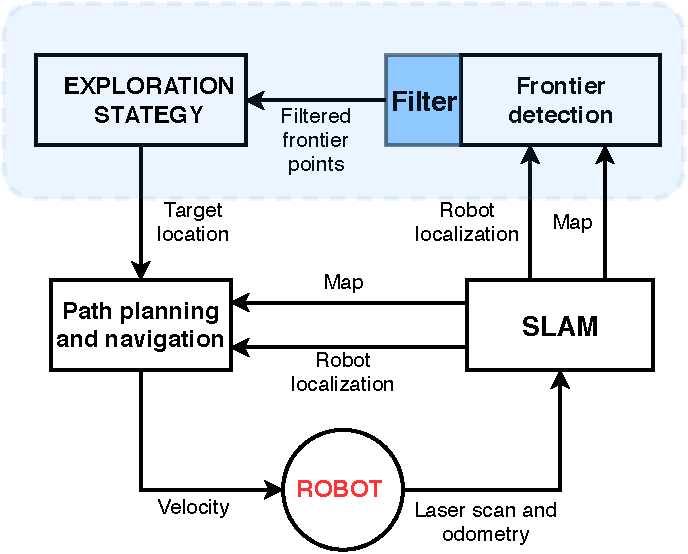
\includegraphics[width=0.6\textwidth]{figures/strategy_one_robot}
		\caption{The overall frontier exploration and mapping process for a single robot that can be easy extended to multi-robot system.}
	\end{figure}
\end{frame}

\section*{Literatura}
\begin{frame}[allowframebreaks]{Literatura}
\printbibliography
\end{frame}

\end{document}